\let\negmedspace\undefined
\let\negthickspace\undefined
\documentclass[journal]{IEEEtran}
\usepackage[a5paper, margin=10mm, onecolumn]{geometry}
\usepackage{tfrupee} % Include tfrupee package

\setlength{\headheight}{1cm} 
\setlength{\headsep}{0mm}     

\usepackage{gvv-book}
\usepackage{gvv}
\usepackage{cite}
\usepackage{amsmath,amssymb,amsfonts,amsthm}
\usepackage{algorithmic}
\usepackage{graphicx}
\usepackage{textcomp}
\usepackage{xcolor}
\usepackage{txfonts}
\usepackage{listings}
\usepackage{enumitem}
\usepackage{mathtools}
\usepackage{gensymb}
\usepackage{comment}
\usepackage[breaklinks=true]{hyperref}
\usepackage{tkz-euclide} 
\usepackage{listings}
\def\inputGnumericTable{}                                 
\usepackage[latin1]{inputenc}                                
\usepackage{color}                                            
\usepackage{array}                                            
\usepackage{longtable}                                       
\usepackage{calc}                                             
\usepackage{multirow}                                         
\usepackage{hhline}                                           
\usepackage{ifthen}                                           
\usepackage{lscape}
\usepackage{circuitikz}
\tikzstyle{block} = [rectangle, draw, fill=blue!20, 
    text width=4em, text centered, rounded corners, minimum height=3em]
\tikzstyle{sum} = [draw, fill=blue!10, circle, minimum size=1cm, node distance=1.5cm]
\tikzstyle{input} = [coordinate]
\tikzstyle{output} = [coordinate]


\begin{document}

\bibliographystyle{IEEEtran}
\vspace{3cm}

\title{4.4.32}
\author{AI25BTECH11036-SNEHAMRUDULA}
 \maketitle
{\let\newpage\relax\maketitle}
\renewcommand{\thefigure}{\theenumi}
\renewcommand{\thetable}{\theenumi}
\setlength{\intextsep}{10pt} 
\numberwithin{equation}{enumi}
\numberwithin{figure}{enumi}
\renewcommand{\thetable}{\theenumi}
\textbf{Question}:\\
\textbf{Q.}\;
Show that the vectors 
$\myvec{1\\-2\\3}$,\;
$\myvec{2\\3\\-4}$ and 
$\myvec{1\\-3\\5}$ are coplanar.
\\ 
\solution \\
\[
\left(\vec{n}^{\,T}\right)\vec{x} = 1
\]
\[
\begin{bmatrix}
1 & -2 & 3 \\
2 & 3 & -4 \\
1 & -3 & 5
\end{bmatrix}
\begin{bmatrix}
l \\ m \\ n
\end{bmatrix}
=
\begin{bmatrix}
1 \\ 1 \\ 1
\end{bmatrix}
\]

The augmented matrix is
\[
\left[
\begin{array}{ccc|c}
1 & -2 & 3 & 1 \\
2 & 3 & -4 & 1 \\
1 & -3 & 5 & 1
\end{array}
\right].
\]

Performing row operations:

\[
R_2 \to R_2 - 2R_1,\quad 
R_3 \to R_3 - R_1
\]

\[
\left[
\begin{array}{ccc|c}
1 & -2 & 3 & 1 \\
0 & 7 & -10 & -1 \\
0 & -1 & 2 & 0
\end{array}
\right]
\]

Swap \(R_2 \leftrightarrow R_3\):

\[
\left[
\begin{array}{ccc|c}
1 & -2 & 3 & 1 \\
0 & -1 & 2 & 0 \\
0 & 7 & -10 & -1
\end{array}
\right]
\]

Now,
\[
R_3 \to R_3 + 7R_2
\]

\[
\left[
\begin{array}{ccc|c}
1 & -2 & 3 & 1 \\
0 & -1 & 2 & 0 \\
0 & 0 & 4 & -1
\end{array}
\right]
\]

---

The coefficient matrix is
\[
\begin{bmatrix}
1 & -2 & 3 \\
0 & -1 & 2 \\
0 & 0 & 4
\end{bmatrix}, 
\quad \operatorname{rank} = 3.
\]

The augmented matrix is
\[
\begin{bmatrix}
1 & -2 & 3 & 1 \\
0 & -1 & 2 & 0 \\
0 & 0 & 4 & -1
\end{bmatrix}, 
\quad \operatorname{rank} = 3.
\]

Since
\[
\operatorname{rank}(\text{Coefficient}) 
= \operatorname{rank}(\text{Augmented}) = 3,
\]
and the number of unknowns is also \(3\), the system has a \textbf{unique solution}.  

\[
\therefore \quad \text{There exists a unique vector } n 
\text{ such that } n^T x = 1 \text{ is the required plane.}
\]
\begin{figure}[h!]
    \centering
    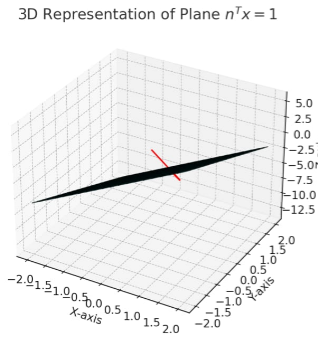
\includegraphics[height=0.5\textheight, keepaspectratio]{fig4.4.32}
    \label{figure_1}
\end{figure}
 
\end{document}
